\chapter{Free Electrons}

\section{The company}
Free Electrons is an engineering company founded in 2004 by Michael Opdenacker, a Linux and Free and Open Source softwares' enthusiast. Since its beginnings, the company offers training services for development in Open Source softwares such as Linux, Yocto Project, Buildroot or Android. It also offers its expertise in embedded Linux development for companies willing, for example, to use Linux in their products, to upstream (publish) drivers in kernel or build a custom system.

%TODO: Add what are the kind of projects the company can work on.

Free Electrons' team is split between two locations in France:
\begin{itemize}
  \item Orange, for General Managers and the accounting,
  \item Toulouse, for the engineering team;
\end{itemize}

Two engineers are also teleworking from Lyon's surroundings.

\section{The team}

%Team Picture?

Free Electrons is proud to have the conviviality of a human-size company with 11 employees and 2 interns:
\begin{itemize}
  \item Michael Opdenacker, founder and CEO,
  \item Maria Llvata, executive director,
  \item Anja Roubin, executive assistant,
  \item Thomas Petazzoni, CTO,
  \item Alexandre Belloni, engineer,
  \item Boris Brezillon, engineer,
  \item Grégory Clément, engineer,
  \item Mylène Josserand, engineer,
  \item Romain Perier, engineer,
  \item Maxime Ripard, engineer,
  \item Antoine Ténart, engineer,
  \item Florent Revest, intern,
  \item Quentin Schulz, intern;
\end{itemize}

\section{Strong focus on Free and Open Source softwares}
Since its creation, Free Electrons is doing its best to contribute to the Free Software community. It does it by releasing all the training materials under free documentation license\footnote{\url{http://free-electrons.com/training/}} and by allocating some time during most of the projects to give back to the community the work done on free softwares.

The company has also a strong preference for clients willing to interact with the free software community by sparing some of project's time on upstreaming modifications to free softwares.

\section{A recognized expertise}
Free Electrons' engineers are well-known in free software's communities, such as Linux kernel and Buildroot, thanks to their tremendous contributions in these projects and also by taking part in famous conferences around the globe, like Embedded Linux Conference\footnote{\url{http://www.embeddedlinuxconference.com/}} or FOSDEM\footnote{\url{https://fosdem.org}}.

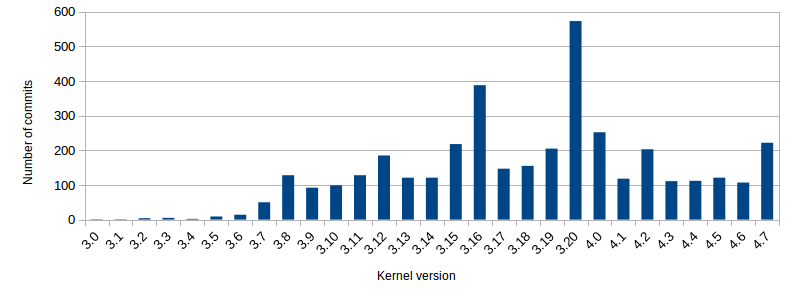
\includegraphics[width=\textwidth]{free-electrons-contributions.png}
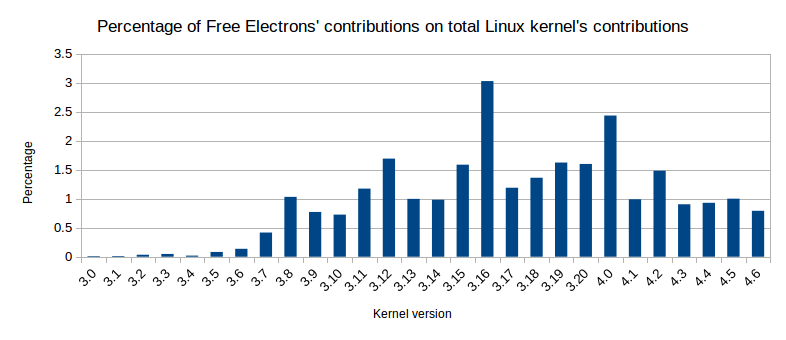
\includegraphics[width=\textwidth]{free-electrons-percentage.png}
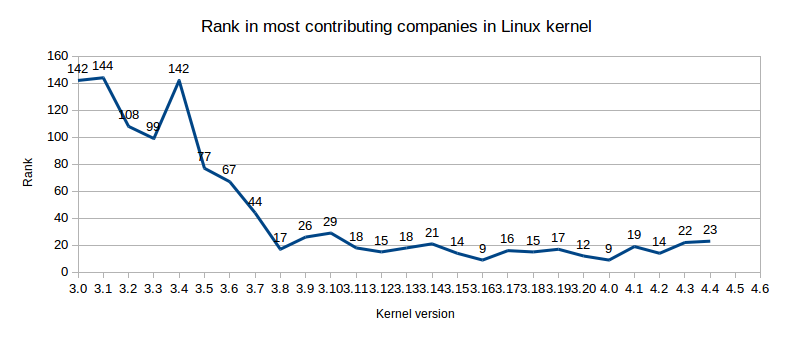
\includegraphics[width=\textwidth]{free-electrons-rank.png}

Being a big contributor often opens great opportunities in the Linux kernel. One of these opportunities is to become a maintainer of a subsystem of the kernel. The Linux kernel is such a big project that it is organized in different parts, called subsystems, and also needs maintainers which take care of a subsystem by validating code being merged to the Linux kernel source code.

Free Electrons has currently 6 maintainers\footnote{\url{https://git.kernel.org/cgit/linux/kernel/git/torvalds/linux.git/tree/MAINTAINERS}} in its engineering team:
\begin{itemize}
\item Alexandre Belloni, maintainer of ATMEL SoCs, Real-Time Clock,
\item Boris Brezillon, maintainer of NAND flash, ATMEL Clocks, Marvell cryptography driver,
\item Grégory Clément, maintainer of Marvell SoCs,
\item Thomas Petazzoni, maintainer of FBTFT Framebuffer drivers, Marvell MVNETA Ethernet driver, Marvell PCI driver,
\item Maxime Ripard, maintainer of Allwinner SoCs, Allwinner A10 DRM drivers, NVMEM framework,
\item Antoine Ténart, maintainer of Annapurna Labs architecture;
\end{itemize}

The company has also big names amongst its clients which assert Free Electrons' expertise:
\begin{itemize}
\item Company 1,
\item Company 2;
\end{itemize}
